% $Id: INF_Poster.tex 7714 2011-08-31 17:34:46Z tkren $
%
% TU Wien - Faculty of Informatics
% poster template
%
% This template is using the beamer document class and beamerposter package, see
% <http://www.ctan.org/tex-archive/macros/latex/contrib/beamer/>
% <http://www.ctan.org/tex-archive/macros/latex/contrib/beamerposter/>
% <http://www-i6.informatik.rwth-aachen.de/~dreuw/latexbeamerposter.php>
%
% For questions and comments send an email to
% Thomas Krennwallner <tkren@kr.tuwien.ac.at>
%

\documentclass[final,hyperref={pdfpagelabels=true}]{beamer}

\makeatletter
  \def\beamer@calltheme#1#2#3{%
    \def\beamer@themelist{#2}
    \@for\beamer@themename:=\beamer@themelist\do
    {\usepackage[{#1}]{\beamer@themelocation/#3\beamer@themename}}}

  \def\usefolder#1{
    \def\beamer@themelocation{#1}
  }
  \def\beamer@themelocation{}

\usefolder{style}

\usepackage{style/TUINFPST}
\usepackage{ragged2e}    %% provides \justifyin
\usepackage{sidecap}     %% for images with side captions
\usepackage{wrapfig}

\title[Software Engineering \& Internet Computing]{Concurrent Programming with\\[.2\baselineskip]Actors and Microservices}
% if you have a long title looking squeezed on the poster, just force
% some distance:
% \title[Computational Intelligence]{%
%   Integration of Conjunctive Queries over \\[0.2\baselineskip]%
%   Description Logics into HEX-Programs %\\[0.2\baselineskip]%
% }
\author[max@irro.at]{Maximilian Irro}
\institute[]{%
  Technische Universit{\"a}t Wien\\[0.25\baselineskip]
  Institut f{\"u}r Information Systems Engineering\\[0.25\baselineskip]
  Arbeitsbereich: Compilers and Languages\\[0.25\baselineskip]
  Betreuer: Ao.Univ.Prof. Dipl.-Ing. Dr. Franz Puntigam
}
\titlegraphic{
\includegraphics[height=52mm]{complang-logo-neu}}
\date[\today]{\today}
\subject{epilog}
\keywords{concurrent programming, actor model, microservices}

%%%%%%%%%%%%%%%%%%%%%%%%%%%%%%%%%%%%%%%%%%%%%%%%%%%%%%%%%%%%%%%%%%%%%%%%%%%%%%%%%%%%%%
% Display a grid to help align images 
%\beamertemplategridbackground[1cm]

% for crop marks, uncomment the following line
%\usepackage[cross,width=88truecm,height=123truecm,center]{crop}

%%%%%%%%%%%%%%%%%%%%%%%%%%%%%%%%%%%%%%%%%%%%%%%%%%%%%%%%%%%%%%%%%%%%%%%%%%%%%%%%%%%%%%

\begin{document}

  % We have a single poster frame.
  \begin{frame}

    \newcommand{\lmodern}{\fontfamily{lmr}\selectfont}

    %\renewcommand\rmdefault{lmr}
    %\renewcommand\sfdefault{lmss}
    %\renewcommand\ttdefault{lmtt}

    %\rmfamily % roman font family

    \begin{columns}[t]
      % ---------------------------------------------------------%
      % Set up a column
      \begin{column}{.45\textwidth}
        \textsf{\textbf{INTRODUCTION}} \\
        \vspace*{\baselineskip}
        {\lmodern\justifying
          Concurrent programming manages multiple concerns of an application or system simultaneously. We investigate two different models for introducing concurrent computational units into software architectures.
        }
      \end{column}
      % ---------------------------------------------------------%
      % end the column

      % ---------------------------------------------------------%
      % Set up a column 
      \begin{column}{.45\textwidth}
        \textsf{\textbf{PROBLEM STATEMENT}} \\
        \vspace*{\baselineskip}
        {\lmodern
          There is yet a gap in the literature that emphasizes the connections between actors and microservices. This work fills this gap by answering these research questions:

          \begin{itemize}
            \item Why do actors and microservices qualify for programming concurrency?
            \item How do the actor and the microservice model facilitate concurrent execution?
            \item What are the expressive capabilities of actors and microservices regarding
  concurrent programming concerns?
            \item How does the performance of actors and microservices compare in a multi-
  core environment relative to a concurrent system scenario?
          \end{itemize}

        }
      \end{column}
      % ---------------------------------------------------------%
      % end the column
    \end{columns}

    \vspace*{2\baselineskip}

    \begin{columns}[t]
    % ---------------------------------------------------------%
    % Set up a column
    \begin{column}{.45\textwidth}
      \textsf{\textbf{ACTOR MODEL}} \\
      \vspace*{\baselineskip}
      {\lmodern
        Lorem ipsum dolor sit amet, consetetur sadipscing elitr, sed diam nonumy eirmod tempor invidunt ut labore et dolore magna aliquyam erat, sed diam voluptua. At vero eos et accusam et justo duo dolores et ea rebum. Stet clita kasd gubergren, no sea takimata sanctus est Lorem ipsum dolor sit amet. 
      }
    \end{column}
    % ---------------------------------------------------------%
    % end the column

    % ---------------------------------------------------------%
    % Set up a column 
    \begin{column}{.45\textwidth}
      \textsf{\textbf{MICROSERVICE PARADIGM}} \\
      \vspace*{\baselineskip}
      {\lmodern
        Lorem ipsum dolor sit amet, consetetur sadipscing elitr, sed diam nonumy eirmod tempor invidunt ut labore et dolore magna aliquyam erat, sed diam voluptua. At vero eos et accusam et justo duo dolores et ea rebum. Stet clita kasd gubergren, no sea takimata sanctus est Lorem ipsum dolor sit amet. 
      }
    \end{column}
    % ---------------------------------------------------------%
    % end the column
  \end{columns}

  \vspace*{2\baselineskip}
  
  \begin{columns}[t]
    % ---------------------------------------------------------%
    % Set up a column
    \begin{column}{.45\textwidth}
      \textsf{\textbf{EXPRESSIVENESS \& CAPABILITIES}} \\
      \vspace*{\baselineskip}
      {\lmodern
        
        Encapsulation

        Communication

        Concurrent Execution

        Scalability
        
      }
    \end{column}
    % ---------------------------------------------------------%
    % end the column

    % ---------------------------------------------------------%
    % Set up a column 
    \begin{column}{.45\textwidth}
      \textsf{\textbf{EFFICIENCY \& BENCHMARK}} \\
      \vspace*{\baselineskip}
      {\lmodern
        Lorem ipsum dolor sit amet, consetetur sadipscing elitr, sed diam nonumy eirmod tempor invidunt ut labore et dolore magna aliquyam erat, sed diam voluptua. At vero eos et accusam et justo duo dolores et ea rebum. Stet clita kasd gubergren, no sea takimata sanctus est Lorem ipsum dolor sit amet. 
      }

      
      \begin{columns}[t]
        \begin{column}{.4\textwidth}
          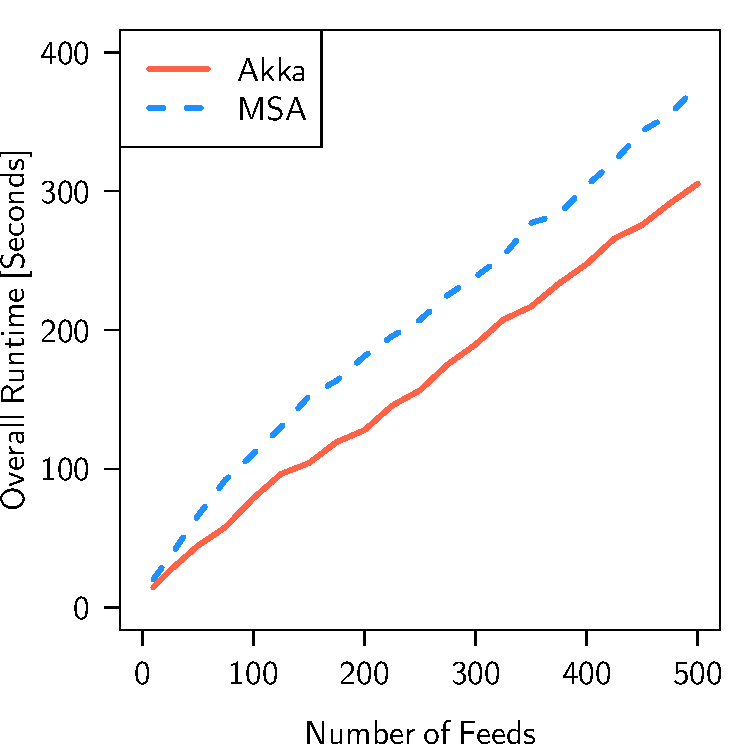
\includegraphics[width=1\textwidth]{graphics/eval-index-overall.pdf}
        \end{column}
        \begin{column}{.05\textwidth}
          % Intentionally left blank
        \end{column}
        \begin{column}{.55\textwidth}
          {\lmodern
            Lorem ipsum dolor sit amet, consetetur sadipscing elitr, sed diam nonumy eirmod tempor invidunt ut labore et dolore magna aliquyam erat, sed diam voluptua.
          }
        \end{column}
      \end{columns}

      \begin{columns}[t]
        \begin{column}{.4\textwidth}
          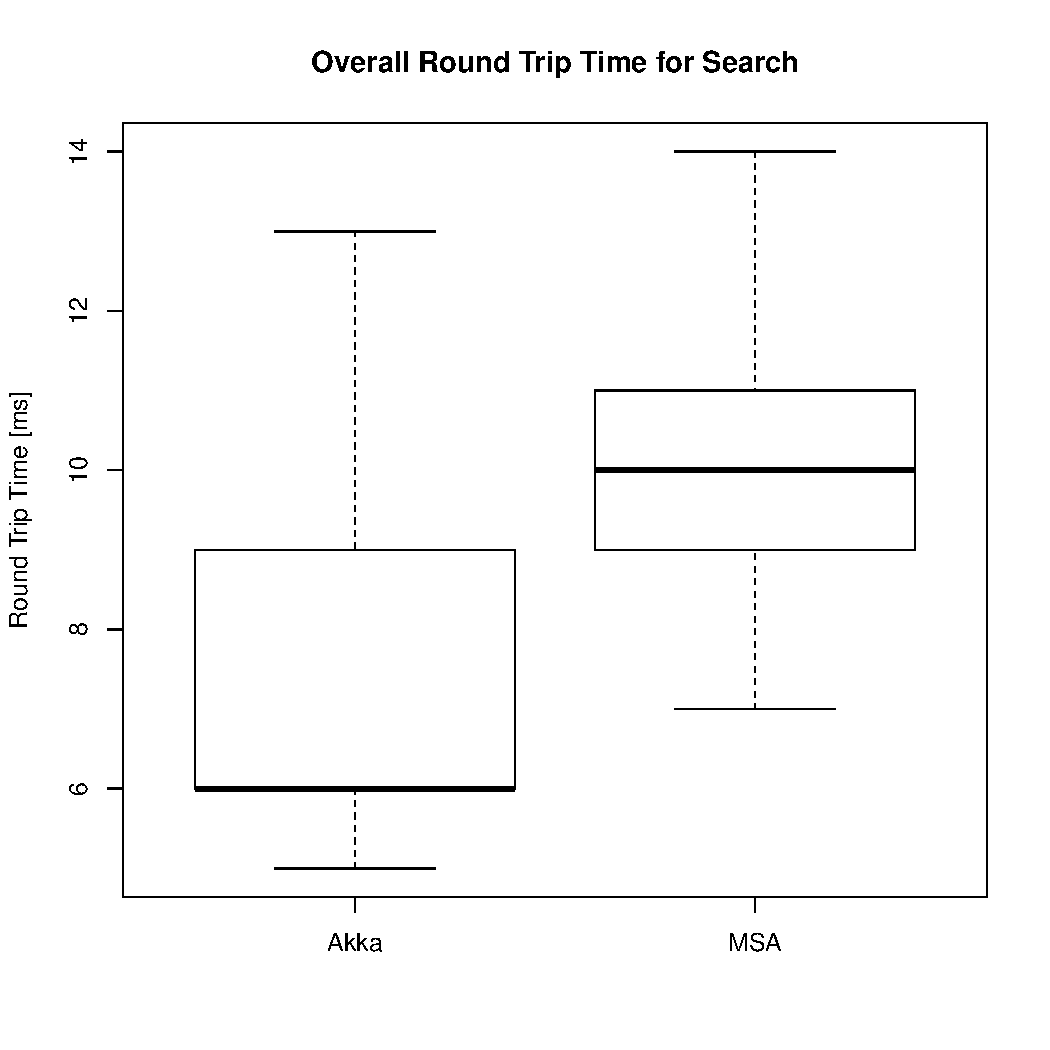
\includegraphics[width=1\textwidth]{graphics/eval-search-rtt-overall.pdf}
        \end{column}
        \begin{column}{.05\textwidth}
          % Intentionally left blank
        \end{column}
        \begin{column}{.55\textwidth}
          {\lmodern
            Lorem ipsum dolor sit amet, consetetur sadipscing elitr, sed diam nonumy eirmod tempor invidunt ut labore et dolore magna aliquyam erat, sed diam voluptua.
          }
        \end{column}
      \end{columns}


    \end{column}
    % ---------------------------------------------------------%
    % end the column
  \end{columns}

\end{frame}

\end{document}

%%% Local Variables:
%%% TeX-PDF-mode: t
%%% TeX-debug-bad-boxes: t
%%% TeX-master: t
%%% TeX-parse-self: t
%%% TeX-auto-save: t
%%% reftex-plug-into-AUCTeX: t
%%% End:
